\section{Développement Code Embarqué}
Dans cette section nous présenterons l'utilisation de NIOS II qui est l'outil de développement de Altera permettant la programmation, compilation et le debug du logiciel que nous implémenterons sur le micro-contrôleur de notre FPGA réalisé précédemment (sous environnement Eclipse).\\

Dans cette partie nous avons utilisé les spécifications du circuit d'interface données dans le cahier des charges pour lier la lecture/écriture des adresses contenant les différents valeurs/données à traiter pour le projet. Si on prend l'exemple de la gestion vérin donnée dans le cahier des charges :

\begin{figure}[h]
    \begin{center}
      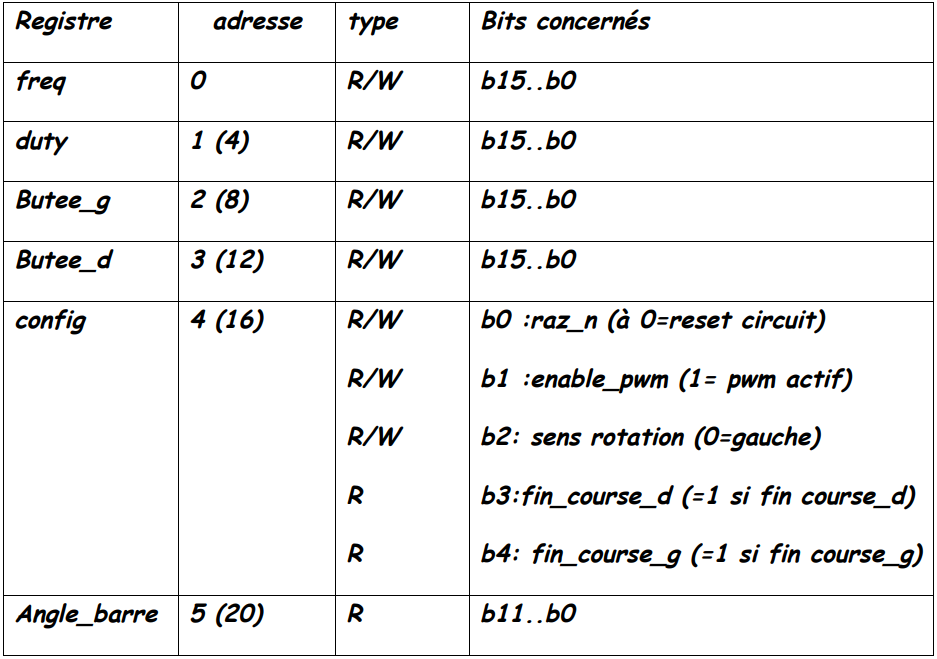
\includegraphics[width=0.6\textwidth]{images/spec_verin.png}
      \caption{Adressage des données Gestion Vérin}
    \end{center}
  \end{figure}

  Il est donc nécessaire dans la partie logicielle embarquée de définir toutes les adresses correspondantes aux fonctions implémentées de tous les blocs matériels. En compilant le projet dans l'environnement Eclipse on peut récupérer les adresses correspondantes des composants dans le fichier "System.h" et les utiliser dans le "main.c" : 

  \begin{figure}[h]
    \begin{center}
      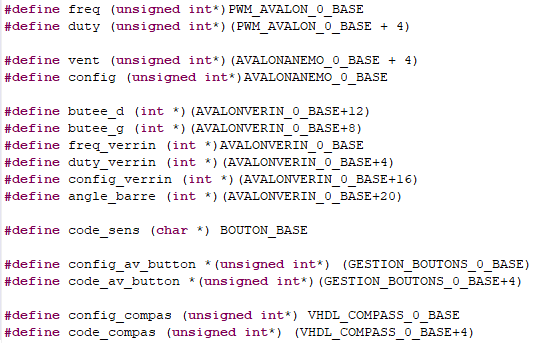
\includegraphics[width=0.6\textwidth]{images/def_spec.png}
      \caption{Implémentation en langage C des adresses matériels}
    \end{center}
  \end{figure}